\documentclass[letterpaper]{article}

% if you need to pass options to natbib, use, e.g.:
% \PassOptionsToPackage{numbers, compress}{natbib}
% before loading nips_2017

% ready for submission
\usepackage[final]{nips_2017}

\usepackage[utf8]{inputenc} % allow utf-8 input
\usepackage[T1]{fontenc}    % use 8-bit T1 fonts
\usepackage{hyperref}       % hyperlinks
\usepackage{url}            % simple URL typesetting
\usepackage{booktabs}       % professional-quality tables
\usepackage{amsfonts}       % blackboard math symbols
\usepackage{graphicx}
\usepackage{lmodern}
\usepackage{nicefrac}       % compact symbols for 1/2, etc.
\usepackage{microtype}      % microtypography

\title{Multitask Object Detection with Dropout and Neural Code Metric Learning}

\author{
  Philip Pham \\
  University of Washington \\
  \href{pmp10@uw.edu}{\texttt{pmp10@uw.edu}} \\
}

\begin{document}

\maketitle

\begin{abstract}
  Using techniques and theory discussed in CSE 547, we try to detect objects in
  images with classification model and retrieve images with metric learning. The
  object detection task was seen as multi-label classification problem. Using
  multitask learning and dropout regularization, a neural network was trained to
  detect objects in patches. The last hidden layer of this network was used for
  neural code metric learning. Neighbors were retrieved with a ball tree.
\end{abstract}

\section{Introduction}

The COCO dataset consists of 330,000 images. Each image is annotated with
bounding boxes which contain objects belonging to one of 80 categories
\citep{coco}. Using this dataset, I explored several techniques covered in CSE
547 including neural networks, non-convex optimization, metric learning, and
nearest neighbor methods.

My objects where:
\begin{itemize}
\item (\emph{object detection}) given an image, extract patches that contain an
  object and classify the object;
\item and (\emph{metric learning}) define a distance metric that compares
  patches such that patches of the same categories are close together, and
  patches of different categories are far apart.
\end{itemize}

In particular, I explored different neural network architecures with various
learning strategies before settling on a multi-layer perceptron model with
dropout. For the metric learning, I attemped to use neural codes
\citep{neural_codes}. Then, the nearest neighbor search is done using a ball
tree.

\section{Methods and Materials}

For object detection, regions were proposed with selective search
\citep{selective_search}. Features for each image were given based on
\cite{fast_rnn}. A fixed length feature vector was extracted for each patch
using pooling \citep{pooling}. For an example of region proposals by selective
search, see Figure \ref{fig:coco_selective_search}.

\begin{figure}
  \centering
  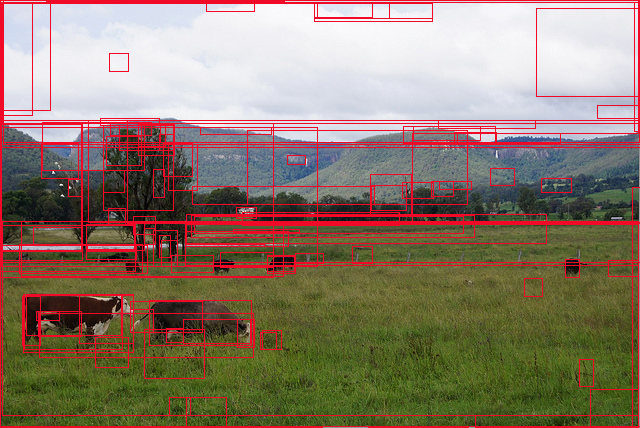
\includegraphics[width=0.7\textwidth]{../hw3/bounding_box_sample.png}
  \caption{Top 128 region proposals by selective search for COCO image 364814.}
  \label{fig:coco_selective_search}
\end{figure}

Using annotations provided by the COCO API, training, validation, and test
datasets were constructed from the patches from the region proposoals with
intersection over union (IoU) over 0.5 with a bouding box from an
annotation. That patch was then labeled with the categories from the annotated
bounding box. The training set consisted of 375,453 patches from 10,000
images. The test set was 74,276 patches from 2,000 images, and the validation
set was 75,620 patches from 2,000 images. Each patch had 11,776 features. From
here, the problem can be seen as a multi-label classification problem. Models
were trained with PyTorch \citep{pytorch}.

The neural codes for the metric learning were extracted from the last hidden
layer of the multi-layer perceptron used for object detection. To find nearest
neighbors, a ball tree from \texttt{sklearn} was used \citep{scikit-learn}.

\section{Results}

The best unweighted mean average precision on the test set was
0.254112. With the
learned metric, the nearest neighbor was of the same category 24\% of the
time.

\subsection{Object Detection}

The multi-layer perceptron with dropout performed best. It consisted of two
hidden layers with 1,024 and 256 units, respectively. At each layer, dropout
with $p = 0.5$ and ReLu activation functions were used.

\subsubsection{Models}

Three types of models were trained for object detection. You can see the
results in Table \ref{tab:model_comparison}. $L2$-regularization parameters
and the number of hidden units were tuned to produce the smallest loss on the
validation dataset. The idea behind using an MLP is that it enables
weight-sharing in the hidden units. One might imagine certain animals or
vehicles have common features that the model could learn together.

\begin{table}[h]
  \centering
  \begin{tabular}{lrr}
\toprule
Model &  Average Precision Score &      Loss \\
\midrule
Linear   &                 0.1750 &  0.1946 \\
  2-layer MLP &                 0.2198 &  0.1824 \\
  MLP with Dropout & 0.2351 & 0.1807 \\
\bottomrule
\end{tabular}
  
  \caption{Metrics are computed against the validation dataset.}
  \label{tab:model_comparison}    
\end{table}

To use multitask learning, multi-label cross entropy was used for the loss
function. The $L2$-regularization parameter $\lambda$ by looking at the
difference between validation and training loss across various training
runs. While there were large differences, regularization was
increased. Eventually, validation loss stopped improving.

To obtain a further improvement, dropout regularization was applied. Dropout is
a form of regularization that randomly zeroes outs a hidden unit during training
\citep{dropout}. Intuitively, this prevents the network from seeing the same
examples and avoids memorizing the training data.

\subsubsection{Model Evaluation}

\subsection{Retrieval of style files}

The style files for NIPS and other conference information are
available on the World Wide Web at
\begin{center}
  \url{http://www.nips.cc/}
\end{center}
The file \verb+nips_2018.pdf+ contains these instructions and
illustrates the various formatting requirements your NIPS paper must
satisfy.

The only supported style file for NIPS 2018 is \verb+nips_2018.sty+,
rewritten for \LaTeXe{}.  \textbf{Previous style files for \LaTeX{}
  2.09, Microsoft Word, and RTF are no longer supported!}

The \LaTeX{} style file contains three optional arguments: \verb+final+,
which creates a camera-ready copy, \verb+preprint+, which creates a
preprint for submission to, e.g., arXiv, and \verb+nonatbib+, which will
not load the \verb+natbib+ package for you in case of package clash.

\paragraph{New preprint option for 2018}
If you wish to post a preprint of your work online, e.g., on arXiv,
using the NIPS style, please use the \verb+preprint+ option. This will
create a nonanonymized version of your work with the text
``Preprint. Work in progress.''  in the footer. This version may be
distributed as you see fit. Please \textbf{do not} use the
\verb+final+ option, which should \textbf{only} be used for papers
accepted to NIPS.

At submission time, please omit the \verb+final+ and \verb+preprint+
options. This will anonymize your submission and add line numbers to aid
review. Please do \emph{not} refer to these line numbers in your paper
as they will be removed during generation of camera-ready copies.

The file \verb+nips_2018.tex+ may be used as a ``shell'' for writing
your paper. All you have to do is replace the author, title, abstract,
and text of the paper with your own.

The formatting instructions contained in these style files are
summarized in Sections \ref{gen_inst}, \ref{headings}, and
\ref{others} below.

\section{General formatting instructions}
\label{gen_inst}

The text must be confined within a rectangle 5.5~inches (33~picas)
wide and 9~inches (54~picas) long. The left margin is 1.5~inch
(9~picas).  Use 10~point type with a vertical spacing (leading) of
11~points.  Times New Roman is the preferred typeface throughout, and
will be selected for you by default.  Paragraphs are separated by
\nicefrac{1}{2}~line space (5.5 points), with no indentation.

The paper title should be 17~point, initial caps/lower case, bold,
centered between two horizontal rules. The top rule should be 4~points
thick and the bottom rule should be 1~point thick. Allow
\nicefrac{1}{4}~inch space above and below the title to rules. All
pages should start at 1~inch (6~picas) from the top of the page.

For the final version, authors' names are set in boldface, and each
name is centered above the corresponding address. The lead author's
name is to be listed first (left-most), and the co-authors' names (if
different address) are set to follow. If there is only one co-author,
list both author and co-author side by side.

Please pay special attention to the instructions in Section \ref{others}
regarding figures, tables, acknowledgments, and references.

\section{Headings: first level}
\label{headings}

All headings should be lower case (except for first word and proper
nouns), flush left, and bold.

First-level headings should be in 12-point type.

\subsection{Headings: second level}

Second-level headings should be in 10-point type.

\subsubsection{Headings: third level}

Third-level headings should be in 10-point type.

\paragraph{Paragraphs}

There is also a \verb+\paragraph+ command available, which sets the
heading in bold, flush left, and inline with the text, with the
heading followed by 1\,em of space.

\section{Citations, figures, tables, references}
\label{others}

These instructions apply to everyone.

\subsection{Citations within the text}

The \verb+natbib+ package will be loaded for you by default.
Citations may be author/year or numeric, as long as you maintain
internal consistency.  As to the format of the references themselves,
any style is acceptable as long as it is used consistently.

The documentation for \verb+natbib+ may be found at
\begin{center}
  \url{http://mirrors.ctan.org/macros/latex/contrib/natbib/natnotes.pdf}
\end{center}
Of note is the command \verb+\citet+, which produces citations
appropriate for use in inline text.  For example,
\begin{verbatim}
   \citet{hasselmo} investigated\dots
\end{verbatim}
produces
\begin{quote}
  Hasselmo, et al.\ (1995) investigated\dots
\end{quote}

If you wish to load the \verb+natbib+ package with options, you may
add the following before loading the \verb+nips_2018+ package:
\begin{verbatim}
   \PassOptionsToPackage{options}{natbib}
\end{verbatim}

If \verb+natbib+ clashes with another package you load, you can add
the optional argument \verb+nonatbib+ when loading the style file:
\begin{verbatim}
   \usepackage[nonatbib]{nips_2018}
\end{verbatim}

As submission is double blind, refer to your own published work in the
third person. That is, use ``In the previous work of Jones et
al.\ [4],'' not ``In our previous work [4].'' If you cite your other
papers that are not widely available (e.g., a journal paper under
review), use anonymous author names in the citation, e.g., an author
of the form ``A.\ Anonymous.''

\subsection{Footnotes}

Footnotes should be used sparingly.  If you do require a footnote,
indicate footnotes with a number\footnote{Sample of the first
  footnote.} in the text. Place the footnotes at the bottom of the
page on which they appear.  Precede the footnote with a horizontal
rule of 2~inches (12~picas).

Note that footnotes are properly typeset \emph{after} punctuation
marks.\footnote{As in this example.}

\subsection{Figures}

\begin{figure}
  \centering
  \fbox{\rule[-.5cm]{0cm}{4cm} \rule[-.5cm]{4cm}{0cm}}
  \caption{Sample figure caption.}
\end{figure}

All artwork must be neat, clean, and legible. Lines should be dark
enough for purposes of reproduction. The figure number and caption
always appear after the figure. Place one line space before the figure
caption and one line space after the figure. The figure caption should
be lower case (except for first word and proper nouns); figures are
numbered consecutively.

You may use color figures.  However, it is best for the figure
captions and the paper body to be legible if the paper is printed in
either black/white or in color.

\subsection{Tables}

All tables must be centered, neat, clean and legible.  The table
number and title always appear before the table.  See
Table~\ref{sample-table}.

Place one line space before the table title, one line space after the
table title, and one line space after the table. The table title must
be lower case (except for first word and proper nouns); tables are
numbered consecutively.

Note that publication-quality tables \emph{do not contain vertical
  rules.} We strongly suggest the use of the \verb+booktabs+ package,
which allows for typesetting high-quality, professional tables:
\begin{center}
  \url{https://www.ctan.org/pkg/booktabs}
\end{center}
This package was used to typeset Table~\ref{sample-table}.

\begin{table}
  \caption{Sample table title}
  \label{sample-table}
  \centering
  \begin{tabular}{lll}
    \toprule
    \multicolumn{2}{c}{Part}                   \\
    \cmidrule(r){1-2}
    Name     & Description     & Size ($\mu$m) \\
    \midrule
    Dendrite & Input terminal  & $\sim$100     \\
    Axon     & Output terminal & $\sim$10      \\
    Soma     & Cell body       & up to $10^6$  \\
    \bottomrule
  \end{tabular}
\end{table}

\section{Final instructions}

Do not change any aspects of the formatting parameters in the style
files.  In particular, do not modify the width or length of the
rectangle the text should fit into, and do not change font sizes
(except perhaps in the \textbf{References} section; see below). Please
note that pages should be numbered.

\section{Preparing PDF files}

Please prepare submission files with paper size ``US Letter,'' and
not, for example, ``A4.''

Fonts were the main cause of problems in the past years. Your PDF file
must only contain Type 1 or Embedded TrueType fonts. Here are a few
instructions to achieve this.

\begin{itemize}

\item You should directly generate PDF files using \verb+pdflatex+.

\item You can check which fonts a PDF files uses.  In Acrobat Reader,
  select the menu Files$>$Document Properties$>$Fonts and select Show
  All Fonts. You can also use the program \verb+pdffonts+ which comes
  with \verb+xpdf+ and is available out-of-the-box on most Linux
  machines.

\item The IEEE has recommendations for generating PDF files whose
  fonts are also acceptable for NIPS. Please see
  \url{http://www.emfield.org/icuwb2010/downloads/IEEE-PDF-SpecV32.pdf}

\item \verb+xfig+ "patterned" shapes are implemented with bitmap
  fonts.  Use "solid" shapes instead.

\item The \verb+\bbold+ package almost always uses bitmap fonts.  You
  should use the equivalent AMS Fonts:
\begin{verbatim}
   \usepackage{amsfonts}
\end{verbatim}
followed by, e.g., \verb+\mathbb{R}+, \verb+\mathbb{N}+, or
\verb+\mathbb{C}+ for $\mathbb{R}$, $\mathbb{N}$ or $\mathbb{C}$.  You
can also use the following workaround for reals, natural and complex:
\begin{verbatim}
   \newcommand{\RR}{I\!\!R} %real numbers
   \newcommand{\Nat}{I\!\!N} %natural numbers
   \newcommand{\CC}{I\!\!\!\!C} %complex numbers
\end{verbatim}
Note that \verb+amsfonts+ is automatically loaded by the
\verb+amssymb+ package.

\end{itemize}

If your file contains type 3 fonts or non embedded TrueType fonts, we
will ask you to fix it.

\subsection{Margins in \LaTeX{}}

Most of the margin problems come from figures positioned by hand using
\verb+\special+ or other commands. We suggest using the command
\verb+\includegraphics+ from the \verb+graphicx+ package. Always
specify the figure width as a multiple of the line width as in the
example below:
\begin{verbatim}
   \usepackage[pdftex]{graphicx} ...
   \includegraphics[width=0.8\linewidth]{myfile.pdf}
\end{verbatim}
See Section 4.4 in the graphics bundle documentation
(\url{http://mirrors.ctan.org/macros/latex/required/graphics/grfguide.pdf})

A number of width problems arise when \LaTeX{} cannot properly
hyphenate a line. Please give LaTeX hyphenation hints using the
\verb+\-+ command when necessary.

\subsubsection*{Acknowledgments}

Use unnumbered third level headings for the acknowledgments. All
acknowledgments go at the end of the paper. Do not include
acknowledgments in the anonymized submission, only in the final paper.

\bibliographystyle{chicago}
\bibliography{references}

\end{document}
